\documentclass[a4paper]{book}
\usepackage{a4wide}
\usepackage{makeidx}
\usepackage{graphicx}
\usepackage{multicol}
\usepackage{float}
\usepackage{listings}
\usepackage{color}
\usepackage{textcomp}
\usepackage{alltt}
\usepackage{times}
\usepackage{ifpdf}
\ifpdf
\usepackage[pdftex,
            pagebackref=true,
            colorlinks=true,
            linkcolor=blue,
            unicode
           ]{hyperref}
\else
\usepackage[ps2pdf,
            pagebackref=true,
            colorlinks=true,
            linkcolor=blue,
            unicode
           ]{hyperref}
\usepackage{pspicture}
\fi
\usepackage[utf8]{inputenc}
\usepackage{doxygen}
\lstset{language=C++,inputencoding=utf8,basicstyle=\footnotesize,breaklines=true,breakatwhitespace=true,tabsize=4,numbers=left }
\makeindex
\setcounter{tocdepth}{3}
\renewcommand{\footrulewidth}{0.4pt}
\begin{document}
\hypersetup{pageanchor=false}
\begin{titlepage}
\vspace*{7cm}
\begin{center}
{\Large LinearC++ \\[1ex]\large 0.0.1 }\\
\vspace*{1cm}
{\large Generated by Doxygen 1.6.3}\\
\vspace*{0.5cm}
{\small Wed Apr 21 17:08:37 2010}\\
\end{center}
\end{titlepage}
\clearemptydoublepage
\pagenumbering{roman}
\tableofcontents
\clearemptydoublepage
\pagenumbering{arabic}
\hypersetup{pageanchor=true}
\chapter{LinearC++ Documentation}
\label{index}\hypertarget{index}{}\hypertarget{index_intro_sec}{}\section{Introduction}\label{index_intro_sec}
This is the reference documentation for LinearC++, a very basic library for doing Linear Algebra using C++. 
\chapter{Class Index}
\section{Class Hierarchy}
This inheritance list is sorted roughly, but not completely, alphabetically:\begin{DoxyCompactList}
\item \contentsline{section}{Matrix}{\pageref{class_matrix}}{}
\begin{DoxyCompactList}
\item \contentsline{section}{ColumnVector}{\pageref{class_column_vector}}{}
\item \contentsline{section}{RowVector}{\pageref{class_row_vector}}{}
\end{DoxyCompactList}
\item \contentsline{section}{MatrixIterator}{\pageref{class_matrix_iterator}}{}
\end{DoxyCompactList}

\chapter{Class Index}
\section{Class List}
Here are the classes, structs, unions and interfaces with brief descriptions:\begin{DoxyCompactList}
\item\contentsline{section}{\hyperlink{class_column_vector}{ColumnVector} (The \hyperlink{class_column_vector}{ColumnVector} class, which inherits from the general \hyperlink{class_matrix}{Matrix} class )}{\pageref{class_column_vector}}{}
\item\contentsline{section}{\hyperlink{class_matrix}{Matrix} (The general \hyperlink{class_matrix}{Matrix} class )}{\pageref{class_matrix}}{}
\item\contentsline{section}{\hyperlink{class_matrix_iterator}{MatrixIterator} (The \hyperlink{class_matrix_iterator}{MatrixIterator} class )}{\pageref{class_matrix_iterator}}{}
\item\contentsline{section}{\hyperlink{class_row_vector}{RowVector} (The \hyperlink{class_row_vector}{RowVector} class, which inherits from the general \hyperlink{class_matrix}{Matrix} class )}{\pageref{class_row_vector}}{}
\end{DoxyCompactList}

\chapter{File Index}
\section{File List}
Here is a list of all files with brief descriptions:\begin{DoxyCompactList}
\item\contentsline{section}{\hyperlink{_matrix_8cpp}{Matrix.cpp} }{\pageref{_matrix_8cpp}}{}
\item\contentsline{section}{\hyperlink{_matrix_8h}{Matrix.h} (This file contains the declarations of the basic Linear Algebra classes and some methods that operate on them )}{\pageref{_matrix_8h}}{}
\item\contentsline{section}{\hyperlink{_matrix_functions_8cpp}{MatrixFunctions.cpp} }{\pageref{_matrix_functions_8cpp}}{}
\item\contentsline{section}{\hyperlink{_matrix_functions_8h}{MatrixFunctions.h} (This file contains the declarations of the basic Linear Algebra classes and some methods that operate on them )}{\pageref{_matrix_functions_8h}}{}
\item\contentsline{section}{\hyperlink{test_8cpp}{test.cpp} }{\pageref{test_8cpp}}{}
\end{DoxyCompactList}

\chapter{Class Documentation}
\hypertarget{class_column_vector}{
\section{ColumnVector Class Reference}
\label{class_column_vector}\index{ColumnVector@{ColumnVector}}
}


The \hyperlink{class_column_vector}{ColumnVector} class, which inherits from the general \hyperlink{class_matrix}{Matrix} class.  




{\ttfamily \#include $<$Matrix.h$>$}



Inherits \hyperlink{class_matrix}{Matrix}.



Collaboration diagram for ColumnVector:\nopagebreak
\begin{figure}[H]
\begin{center}
\leavevmode
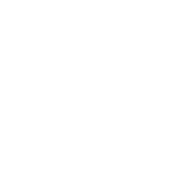
\includegraphics[width=124pt]{class_column_vector__coll__graph}
\end{center}
\end{figure}
\subsection*{Public Member Functions}
\begin{DoxyCompactItemize}
\item 
\hyperlink{class_column_vector_a080508988b684290b2a0123a923a1e08}{ColumnVector} (int r)
\begin{DoxyCompactList}\small\item\em Creates a \hyperlink{class_column_vector}{ColumnVector} of the specified length. \item\end{DoxyCompactList}\item 
\hyperlink{class_column_vector_a51a68a454f01918fd4bc1736ac0d4264}{ColumnVector} (std::vector$<$ double $>$ \&a)
\begin{DoxyCompactList}\small\item\em Creates a \hyperlink{class_column_vector}{ColumnVector} from a vector of doubles. \item\end{DoxyCompactList}\item 
\hyperlink{class_column_vector_aa0b9560305d34dd819e7913a811f3336}{ColumnVector} (double $\ast$a, int size)
\begin{DoxyCompactList}\small\item\em Creates a \hyperlink{class_column_vector}{ColumnVector} from an array of doubles, with the size of the array as the second argument. \item\end{DoxyCompactList}\item 
\hyperlink{class_column_vector_a3fae5c07b5b805aa05da3c9952838892}{ColumnVector} (\hyperlink{class_matrix}{Matrix} a)
\begin{DoxyCompactList}\small\item\em Creates a \hyperlink{class_column_vector}{ColumnVector} from a \hyperlink{class_matrix}{Matrix}. \item\end{DoxyCompactList}\item 
double \hyperlink{class_column_vector_a66329a870ee70b5cd93879d3be247b21}{length} ()
\begin{DoxyCompactList}\small\item\em Calculates and returns the length of the vector. \item\end{DoxyCompactList}\item 
void \hyperlink{class_column_vector_a0e67b7831d9d4c02691056a72abc6975}{appendCol} ()
\begin{DoxyCompactList}\small\item\em This method is undefined for a \hyperlink{class_column_vector}{ColumnVector} since a \hyperlink{class_column_vector}{ColumnVector} can only have one column. \item\end{DoxyCompactList}\end{DoxyCompactItemize}


\subsection{Detailed Description}
The \hyperlink{class_column_vector}{ColumnVector} class, which inherits from the general \hyperlink{class_matrix}{Matrix} class. If you want to do vector-\/specific operations like get the length of the vector, use this class instead of the \hyperlink{class_matrix}{Matrix} class. 

\subsection{Constructor \& Destructor Documentation}
\hypertarget{class_column_vector_a080508988b684290b2a0123a923a1e08}{
\index{ColumnVector@{ColumnVector}!ColumnVector@{ColumnVector}}
\index{ColumnVector@{ColumnVector}!ColumnVector@{ColumnVector}}
\subsubsection[{ColumnVector}]{\setlength{\rightskip}{0pt plus 5cm}ColumnVector::ColumnVector (int {\em r})\hspace{0.3cm}{\ttfamily  \mbox{[}inline, explicit\mbox{]}}}}
\label{class_column_vector_a080508988b684290b2a0123a923a1e08}


Creates a \hyperlink{class_column_vector}{ColumnVector} of the specified length. 

\hypertarget{class_column_vector_a51a68a454f01918fd4bc1736ac0d4264}{
\index{ColumnVector@{ColumnVector}!ColumnVector@{ColumnVector}}
\index{ColumnVector@{ColumnVector}!ColumnVector@{ColumnVector}}
\subsubsection[{ColumnVector}]{\setlength{\rightskip}{0pt plus 5cm}ColumnVector::ColumnVector (std::vector$<$ double $>$ \& {\em a})}}
\label{class_column_vector_a51a68a454f01918fd4bc1736ac0d4264}


Creates a \hyperlink{class_column_vector}{ColumnVector} from a vector of doubles. 

\hypertarget{class_column_vector_aa0b9560305d34dd819e7913a811f3336}{
\index{ColumnVector@{ColumnVector}!ColumnVector@{ColumnVector}}
\index{ColumnVector@{ColumnVector}!ColumnVector@{ColumnVector}}
\subsubsection[{ColumnVector}]{\setlength{\rightskip}{0pt plus 5cm}ColumnVector::ColumnVector (double $\ast$ {\em a}, \/  int {\em size})}}
\label{class_column_vector_aa0b9560305d34dd819e7913a811f3336}


Creates a \hyperlink{class_column_vector}{ColumnVector} from an array of doubles, with the size of the array as the second argument. 

\hypertarget{class_column_vector_a3fae5c07b5b805aa05da3c9952838892}{
\index{ColumnVector@{ColumnVector}!ColumnVector@{ColumnVector}}
\index{ColumnVector@{ColumnVector}!ColumnVector@{ColumnVector}}
\subsubsection[{ColumnVector}]{\setlength{\rightskip}{0pt plus 5cm}ColumnVector::ColumnVector ({\bf Matrix} {\em a})\hspace{0.3cm}{\ttfamily  \mbox{[}inline\mbox{]}}}}
\label{class_column_vector_a3fae5c07b5b805aa05da3c9952838892}


Creates a \hyperlink{class_column_vector}{ColumnVector} from a \hyperlink{class_matrix}{Matrix}. 



\subsection{Member Function Documentation}
\hypertarget{class_column_vector_a0e67b7831d9d4c02691056a72abc6975}{
\index{ColumnVector@{ColumnVector}!appendCol@{appendCol}}
\index{appendCol@{appendCol}!ColumnVector@{ColumnVector}}
\subsubsection[{appendCol}]{\setlength{\rightskip}{0pt plus 5cm}void ColumnVector::appendCol ()}}
\label{class_column_vector_a0e67b7831d9d4c02691056a72abc6975}


This method is undefined for a \hyperlink{class_column_vector}{ColumnVector} since a \hyperlink{class_column_vector}{ColumnVector} can only have one column. 

\hypertarget{class_column_vector_a66329a870ee70b5cd93879d3be247b21}{
\index{ColumnVector@{ColumnVector}!length@{length}}
\index{length@{length}!ColumnVector@{ColumnVector}}
\subsubsection[{length}]{\setlength{\rightskip}{0pt plus 5cm}double ColumnVector::length ()}}
\label{class_column_vector_a66329a870ee70b5cd93879d3be247b21}


Calculates and returns the length of the vector. 



The documentation for this class was generated from the following files:\begin{DoxyCompactItemize}
\item 
\hyperlink{_matrix_8h}{Matrix.h}\item 
\hyperlink{_matrix_8cpp}{Matrix.cpp}\end{DoxyCompactItemize}

\hypertarget{class_matrix}{
\section{Matrix Class Reference}
\label{class_matrix}\index{Matrix@{Matrix}}
}


The general \hyperlink{class_matrix}{Matrix} class.  




{\ttfamily \#include $<$Matrix.h$>$}



Inherited by \hyperlink{class_column_vector}{ColumnVector}, and \hyperlink{class_row_vector}{RowVector}.

\subsection*{Public Member Functions}
\begin{DoxyCompactItemize}
\item 
\hyperlink{class_matrix_a07a3cee5bc286ca27ceffe81ce5a2d01}{Matrix} (int r, int c)
\begin{DoxyCompactList}\small\item\em Creates a zero matrix of the given size. \item\end{DoxyCompactList}\item 
int \hyperlink{class_matrix_af238216c5c5ebf0a80e37bba96c99662}{rows} () const 
\begin{DoxyCompactList}\small\item\em Returns the number of rows in the matrix. \item\end{DoxyCompactList}\item 
int \hyperlink{class_matrix_ac9586a9d7bba127292ce84b1e8ee9cc1}{cols} () const 
\begin{DoxyCompactList}\small\item\em Returns the number of columns in the matrix. \item\end{DoxyCompactList}\item 
\hyperlink{class_matrix_a0db283ef4ea2660f8d0c1b58f9e74f49}{Matrix} (std::vector$<$ std::vector$<$ double $>$ $>$ \&a)
\begin{DoxyCompactList}\small\item\em Creates a \hyperlink{class_matrix}{Matrix} object from a 2d vector of doubles. \item\end{DoxyCompactList}\item 
\hyperlink{class_matrix_a3179cefb929e09cbdc95d143e1d9e3d2}{Matrix} (double $\ast$a, int rows, int cols)
\begin{DoxyCompactList}\small\item\em Creates a \hyperlink{class_matrix}{Matrix} object from an array of doubles. \item\end{DoxyCompactList}\item 
\hyperlink{class_matrix}{Matrix} \& \hyperlink{class_matrix_a375fc575a7e042d0eed3d76c7470e59f}{populateRandom} ()
\begin{DoxyCompactList}\small\item\em Populates the matrix with random integers in the range 0-\/9. \item\end{DoxyCompactList}\item 
\hyperlink{class_matrix}{Matrix} \& \hyperlink{class_matrix_abeb4729f525e85a0f1f516675677e105}{populateSymmetric} ()
\begin{DoxyCompactList}\small\item\em Populates the matrix with random integers in the range 0-\/9. \item\end{DoxyCompactList}\item 
\hyperlink{class_matrix}{Matrix} \& \hyperlink{class_matrix_a0ee71091770a4e83e54860f291ef1b7d}{populateIdentity} ()
\begin{DoxyCompactList}\small\item\em Makes this matrix an identity matrix. \item\end{DoxyCompactList}\item 
\hyperlink{class_matrix}{Matrix} \hyperlink{class_matrix_ae23f817021383e3c8636a714dcba1d21}{transpose} ()
\begin{DoxyCompactList}\small\item\em Returns a \hyperlink{class_matrix}{Matrix} object that is the transpose of the current \hyperlink{class_matrix}{Matrix}. \item\end{DoxyCompactList}\item 
\hyperlink{class_matrix}{Matrix} \hyperlink{class_matrix_ac4f5e7d4bb1bfd6586bd3384bd2a02b0}{inverse} ()
\begin{DoxyCompactList}\small\item\em Returns a \hyperlink{class_matrix}{Matrix} object that is the inverse of the current \hyperlink{class_matrix}{Matrix}. \item\end{DoxyCompactList}\item 
double \hyperlink{class_matrix_ace95025dd985ddaa6c1ed72e8b464a0a}{det} ()
\begin{DoxyCompactList}\small\item\em Returns the determinant of the \hyperlink{class_matrix}{Matrix}. \item\end{DoxyCompactList}\item 
double \hyperlink{class_matrix_af7403d8c02553a4fba253380e4e0bc40}{trace} ()
\begin{DoxyCompactList}\small\item\em Returns the trace of the \hyperlink{class_matrix}{Matrix}. \item\end{DoxyCompactList}\item 
double \& \hyperlink{class_matrix_a3d361fded5f8992d2202894ca141eb72}{operator()} (int i, int j) const 
\begin{DoxyCompactList}\small\item\em This allows you to access the elements in the matrix using subscripts. \item\end{DoxyCompactList}\item 
virtual void \hyperlink{class_matrix_a20c175983a6b23a83fccfe8f726b3b07}{appendRow} (\hyperlink{class_matrix}{Matrix} \&b)
\begin{DoxyCompactList}\small\item\em Adds a row to the current \hyperlink{class_matrix}{Matrix} object. \item\end{DoxyCompactList}\item 
virtual void \hyperlink{class_matrix_a55104cb3fcf93a887ac713955fc0f5c9}{appendRow} (double $\ast$r, int size)
\begin{DoxyCompactList}\small\item\em Same as appendRow, but takes an array as the first argument and the length of the array as the second argument. \item\end{DoxyCompactList}\item 
virtual void \hyperlink{class_matrix_a934b0686d9a2b971e9740b9a29224a54}{appendRow} (std::vector$<$ double $>$ \&r)
\begin{DoxyCompactList}\small\item\em Same as appendRow, but takes a vector. \item\end{DoxyCompactList}\item 
virtual void \hyperlink{class_matrix_a6d7061bb02cf34f6c79a01ff25b41e84}{appendCol} (\hyperlink{class_matrix}{Matrix} \&b)
\begin{DoxyCompactList}\small\item\em Adds a column to the current \hyperlink{class_matrix}{Matrix} object. \item\end{DoxyCompactList}\item 
virtual void \hyperlink{class_matrix_aae8efe9de26740e3c953e43de55963b2}{appendCol} (double $\ast$r, int size)
\begin{DoxyCompactList}\small\item\em Same as appendCol, but takes an array as the first argument and the length of the array as the second argument. \item\end{DoxyCompactList}\item 
virtual void \hyperlink{class_matrix_a726f7ae83284c090af821752628974af}{appendCol} (std::vector$<$ double $>$ \&r)
\begin{DoxyCompactList}\small\item\em Same as appendCol, but takes a vector. \item\end{DoxyCompactList}\item 
void \hyperlink{class_matrix_ac0e73d5e98817e12b82a3f626c8343de}{swapRows} (int rowA, int rowB)
\begin{DoxyCompactList}\small\item\em Swaps the given rows in the \hyperlink{class_matrix}{Matrix}. \item\end{DoxyCompactList}\item 
void \hyperlink{class_matrix_a505f924baa7c236280751499da56ecee}{swapCols} (int colA, int colB)
\begin{DoxyCompactList}\small\item\em Swaps the given cols in the \hyperlink{class_matrix}{Matrix}. \item\end{DoxyCompactList}\item 
\hyperlink{class_matrix_iterator}{MatrixIterator} \hyperlink{class_matrix_a8969f52f950b124d5a40128c3df11efe}{begin} () const 
\begin{DoxyCompactList}\small\item\em Returns an iterator to the beginning of the matrix. \item\end{DoxyCompactList}\item 
\hyperlink{class_matrix_iterator}{MatrixIterator} \hyperlink{class_matrix_aa6e886dcd213fdf5c54743f3b8ac7209}{end} () const 
\begin{DoxyCompactList}\small\item\em Returns an iterator to one past the end of the matrix. \item\end{DoxyCompactList}\end{DoxyCompactItemize}
\subsection*{Protected Attributes}
\begin{DoxyCompactItemize}
\item 
std::vector$<$ std::vector$<$ double $>$ $>$ \hyperlink{class_matrix_adab4557133e13b08ae470a8e5df7b99c}{data}
\begin{DoxyCompactList}\small\item\em Here's where the matrix is actually stored. \item\end{DoxyCompactList}\end{DoxyCompactItemize}


\subsection{Detailed Description}
The general \hyperlink{class_matrix}{Matrix} class. Defines several methods to create and populate matrices. Each element in a matrix is a double.

If you really want a vector instead, use \hyperlink{class_row_vector}{RowVector} or \hyperlink{class_column_vector}{ColumnVector}. This allows for additional operations such as length(). 

\subsection{Constructor \& Destructor Documentation}
\hypertarget{class_matrix_a07a3cee5bc286ca27ceffe81ce5a2d01}{
\index{Matrix@{Matrix}!Matrix@{Matrix}}
\index{Matrix@{Matrix}!Matrix@{Matrix}}
\subsubsection[{Matrix}]{\setlength{\rightskip}{0pt plus 5cm}Matrix::Matrix (int {\em r}, \/  int {\em c})}}
\label{class_matrix_a07a3cee5bc286ca27ceffe81ce5a2d01}


Creates a zero matrix of the given size. 

Will throw an error if you try to create a matrix of negative dimensions. \hypertarget{class_matrix_a0db283ef4ea2660f8d0c1b58f9e74f49}{
\index{Matrix@{Matrix}!Matrix@{Matrix}}
\index{Matrix@{Matrix}!Matrix@{Matrix}}
\subsubsection[{Matrix}]{\setlength{\rightskip}{0pt plus 5cm}Matrix::Matrix (std::vector$<$ std::vector$<$ double $>$ $>$ \& {\em a})}}
\label{class_matrix_a0db283ef4ea2660f8d0c1b58f9e74f49}


Creates a \hyperlink{class_matrix}{Matrix} object from a 2d vector of doubles. 

\hypertarget{class_matrix_a3179cefb929e09cbdc95d143e1d9e3d2}{
\index{Matrix@{Matrix}!Matrix@{Matrix}}
\index{Matrix@{Matrix}!Matrix@{Matrix}}
\subsubsection[{Matrix}]{\setlength{\rightskip}{0pt plus 5cm}Matrix::Matrix (double $\ast$ {\em a}, \/  int {\em rows}, \/  int {\em cols})}}
\label{class_matrix_a3179cefb929e09cbdc95d143e1d9e3d2}


Creates a \hyperlink{class_matrix}{Matrix} object from an array of doubles. 

The array should be a 1-\/d array, even if it is a matrix. The \# of rows and \# of columns are then passed as the second and third parameter. For example:


\begin{DoxyCode}
            // Here we're creating a 2x2 identity matrix:
            double v[] = {1,0,0,1};
            Matrix A(v,2,2);
            
            // print out the matrix:
            cout << A << endl;
\end{DoxyCode}
 

\subsection{Member Function Documentation}
\hypertarget{class_matrix_a726f7ae83284c090af821752628974af}{
\index{Matrix@{Matrix}!appendCol@{appendCol}}
\index{appendCol@{appendCol}!Matrix@{Matrix}}
\subsubsection[{appendCol}]{\setlength{\rightskip}{0pt plus 5cm}void Matrix::appendCol (std::vector$<$ double $>$ \& {\em r})\hspace{0.3cm}{\ttfamily  \mbox{[}virtual\mbox{]}}}}
\label{class_matrix_a726f7ae83284c090af821752628974af}


Same as appendCol, but takes a vector. 

\hypertarget{class_matrix_aae8efe9de26740e3c953e43de55963b2}{
\index{Matrix@{Matrix}!appendCol@{appendCol}}
\index{appendCol@{appendCol}!Matrix@{Matrix}}
\subsubsection[{appendCol}]{\setlength{\rightskip}{0pt plus 5cm}void Matrix::appendCol (double $\ast$ {\em r}, \/  int {\em size})\hspace{0.3cm}{\ttfamily  \mbox{[}virtual\mbox{]}}}}
\label{class_matrix_aae8efe9de26740e3c953e43de55963b2}


Same as appendCol, but takes an array as the first argument and the length of the array as the second argument. 

\hypertarget{class_matrix_a6d7061bb02cf34f6c79a01ff25b41e84}{
\index{Matrix@{Matrix}!appendCol@{appendCol}}
\index{appendCol@{appendCol}!Matrix@{Matrix}}
\subsubsection[{appendCol}]{\setlength{\rightskip}{0pt plus 5cm}void Matrix::appendCol ({\bf Matrix} \& {\em b})\hspace{0.3cm}{\ttfamily  \mbox{[}virtual\mbox{]}}}}
\label{class_matrix_a6d7061bb02cf34f6c79a01ff25b41e84}


Adds a column to the current \hyperlink{class_matrix}{Matrix} object. 

The new column must be the same length as all the other column in the matrix. \hypertarget{class_matrix_a934b0686d9a2b971e9740b9a29224a54}{
\index{Matrix@{Matrix}!appendRow@{appendRow}}
\index{appendRow@{appendRow}!Matrix@{Matrix}}
\subsubsection[{appendRow}]{\setlength{\rightskip}{0pt plus 5cm}void Matrix::appendRow (std::vector$<$ double $>$ \& {\em r})\hspace{0.3cm}{\ttfamily  \mbox{[}virtual\mbox{]}}}}
\label{class_matrix_a934b0686d9a2b971e9740b9a29224a54}


Same as appendRow, but takes a vector. 

\hypertarget{class_matrix_a55104cb3fcf93a887ac713955fc0f5c9}{
\index{Matrix@{Matrix}!appendRow@{appendRow}}
\index{appendRow@{appendRow}!Matrix@{Matrix}}
\subsubsection[{appendRow}]{\setlength{\rightskip}{0pt plus 5cm}void Matrix::appendRow (double $\ast$ {\em r}, \/  int {\em size})\hspace{0.3cm}{\ttfamily  \mbox{[}virtual\mbox{]}}}}
\label{class_matrix_a55104cb3fcf93a887ac713955fc0f5c9}


Same as appendRow, but takes an array as the first argument and the length of the array as the second argument. 

\hypertarget{class_matrix_a20c175983a6b23a83fccfe8f726b3b07}{
\index{Matrix@{Matrix}!appendRow@{appendRow}}
\index{appendRow@{appendRow}!Matrix@{Matrix}}
\subsubsection[{appendRow}]{\setlength{\rightskip}{0pt plus 5cm}void Matrix::appendRow ({\bf Matrix} \& {\em b})\hspace{0.3cm}{\ttfamily  \mbox{[}virtual\mbox{]}}}}
\label{class_matrix_a20c175983a6b23a83fccfe8f726b3b07}


Adds a row to the current \hyperlink{class_matrix}{Matrix} object. 

The new row must be the same length as all the other rows in the matrix. \hypertarget{class_matrix_a8969f52f950b124d5a40128c3df11efe}{
\index{Matrix@{Matrix}!begin@{begin}}
\index{begin@{begin}!Matrix@{Matrix}}
\subsubsection[{begin}]{\setlength{\rightskip}{0pt plus 5cm}{\bf MatrixIterator} Matrix::begin () const}}
\label{class_matrix_a8969f52f950b124d5a40128c3df11efe}


Returns an iterator to the beginning of the matrix. 

\hypertarget{class_matrix_ac9586a9d7bba127292ce84b1e8ee9cc1}{
\index{Matrix@{Matrix}!cols@{cols}}
\index{cols@{cols}!Matrix@{Matrix}}
\subsubsection[{cols}]{\setlength{\rightskip}{0pt plus 5cm}int Matrix::cols () const}}
\label{class_matrix_ac9586a9d7bba127292ce84b1e8ee9cc1}


Returns the number of columns in the matrix. 

\hypertarget{class_matrix_ace95025dd985ddaa6c1ed72e8b464a0a}{
\index{Matrix@{Matrix}!det@{det}}
\index{det@{det}!Matrix@{Matrix}}
\subsubsection[{det}]{\setlength{\rightskip}{0pt plus 5cm}double Matrix::det ()}}
\label{class_matrix_ace95025dd985ddaa6c1ed72e8b464a0a}


Returns the determinant of the \hyperlink{class_matrix}{Matrix}. 

\hypertarget{class_matrix_aa6e886dcd213fdf5c54743f3b8ac7209}{
\index{Matrix@{Matrix}!end@{end}}
\index{end@{end}!Matrix@{Matrix}}
\subsubsection[{end}]{\setlength{\rightskip}{0pt plus 5cm}{\bf MatrixIterator} Matrix::end () const}}
\label{class_matrix_aa6e886dcd213fdf5c54743f3b8ac7209}


Returns an iterator to one past the end of the matrix. 

\hypertarget{class_matrix_ac4f5e7d4bb1bfd6586bd3384bd2a02b0}{
\index{Matrix@{Matrix}!inverse@{inverse}}
\index{inverse@{inverse}!Matrix@{Matrix}}
\subsubsection[{inverse}]{\setlength{\rightskip}{0pt plus 5cm}{\bf Matrix} Matrix::inverse ()}}
\label{class_matrix_ac4f5e7d4bb1bfd6586bd3384bd2a02b0}


Returns a \hyperlink{class_matrix}{Matrix} object that is the inverse of the current \hyperlink{class_matrix}{Matrix}. 

\hypertarget{class_matrix_a3d361fded5f8992d2202894ca141eb72}{
\index{Matrix@{Matrix}!operator()@{operator()}}
\index{operator()@{operator()}!Matrix@{Matrix}}
\subsubsection[{operator()}]{\setlength{\rightskip}{0pt plus 5cm}double \& Matrix::operator() (int {\em i}, \/  int {\em j}) const}}
\label{class_matrix_a3d361fded5f8992d2202894ca141eb72}


This allows you to access the elements in the matrix using subscripts. 

Example: 
\begin{DoxyCode}
                Matrix m(10,10);        // create a 10x10 Matrix
                m(0,0) = 10;            // set it's first element to 10
                cout << m(9,9) << endl; // print it's last element
\end{DoxyCode}
 This is similar to MATLAB's notation for matrices, but our matrices are zero-\/indexed. Data is accessed via (row\#, colunm\#). \hypertarget{class_matrix_a0ee71091770a4e83e54860f291ef1b7d}{
\index{Matrix@{Matrix}!populateIdentity@{populateIdentity}}
\index{populateIdentity@{populateIdentity}!Matrix@{Matrix}}
\subsubsection[{populateIdentity}]{\setlength{\rightskip}{0pt plus 5cm}{\bf Matrix} \& Matrix::populateIdentity ()}}
\label{class_matrix_a0ee71091770a4e83e54860f291ef1b7d}


Makes this matrix an identity matrix. 

Throws an error if this is not a square matrix. \hypertarget{class_matrix_a375fc575a7e042d0eed3d76c7470e59f}{
\index{Matrix@{Matrix}!populateRandom@{populateRandom}}
\index{populateRandom@{populateRandom}!Matrix@{Matrix}}
\subsubsection[{populateRandom}]{\setlength{\rightskip}{0pt plus 5cm}{\bf Matrix} \& Matrix::populateRandom ()}}
\label{class_matrix_a375fc575a7e042d0eed3d76c7470e59f}


Populates the matrix with random integers in the range 0-\/9. 

Guaranteed to be non-\/singular if the \hyperlink{class_matrix}{Matrix} is square. \hypertarget{class_matrix_abeb4729f525e85a0f1f516675677e105}{
\index{Matrix@{Matrix}!populateSymmetric@{populateSymmetric}}
\index{populateSymmetric@{populateSymmetric}!Matrix@{Matrix}}
\subsubsection[{populateSymmetric}]{\setlength{\rightskip}{0pt plus 5cm}{\bf Matrix} \& Matrix::populateSymmetric ()}}
\label{class_matrix_abeb4729f525e85a0f1f516675677e105}


Populates the matrix with random integers in the range 0-\/9. 

Ensures that the matrix is symmetric. Guaranteed to be non-\/singular. \hypertarget{class_matrix_af238216c5c5ebf0a80e37bba96c99662}{
\index{Matrix@{Matrix}!rows@{rows}}
\index{rows@{rows}!Matrix@{Matrix}}
\subsubsection[{rows}]{\setlength{\rightskip}{0pt plus 5cm}int Matrix::rows () const}}
\label{class_matrix_af238216c5c5ebf0a80e37bba96c99662}


Returns the number of rows in the matrix. 

\hypertarget{class_matrix_a505f924baa7c236280751499da56ecee}{
\index{Matrix@{Matrix}!swapCols@{swapCols}}
\index{swapCols@{swapCols}!Matrix@{Matrix}}
\subsubsection[{swapCols}]{\setlength{\rightskip}{0pt plus 5cm}void Matrix::swapCols (int {\em colA}, \/  int {\em colB})}}
\label{class_matrix_a505f924baa7c236280751499da56ecee}


Swaps the given cols in the \hyperlink{class_matrix}{Matrix}. 

\hypertarget{class_matrix_ac0e73d5e98817e12b82a3f626c8343de}{
\index{Matrix@{Matrix}!swapRows@{swapRows}}
\index{swapRows@{swapRows}!Matrix@{Matrix}}
\subsubsection[{swapRows}]{\setlength{\rightskip}{0pt plus 5cm}void Matrix::swapRows (int {\em rowA}, \/  int {\em rowB})}}
\label{class_matrix_ac0e73d5e98817e12b82a3f626c8343de}


Swaps the given rows in the \hyperlink{class_matrix}{Matrix}. 

\hypertarget{class_matrix_af7403d8c02553a4fba253380e4e0bc40}{
\index{Matrix@{Matrix}!trace@{trace}}
\index{trace@{trace}!Matrix@{Matrix}}
\subsubsection[{trace}]{\setlength{\rightskip}{0pt plus 5cm}double Matrix::trace ()}}
\label{class_matrix_af7403d8c02553a4fba253380e4e0bc40}


Returns the trace of the \hyperlink{class_matrix}{Matrix}. 

\hypertarget{class_matrix_ae23f817021383e3c8636a714dcba1d21}{
\index{Matrix@{Matrix}!transpose@{transpose}}
\index{transpose@{transpose}!Matrix@{Matrix}}
\subsubsection[{transpose}]{\setlength{\rightskip}{0pt plus 5cm}{\bf Matrix} Matrix::transpose ()}}
\label{class_matrix_ae23f817021383e3c8636a714dcba1d21}


Returns a \hyperlink{class_matrix}{Matrix} object that is the transpose of the current \hyperlink{class_matrix}{Matrix}. 



\subsection{Member Data Documentation}
\hypertarget{class_matrix_adab4557133e13b08ae470a8e5df7b99c}{
\index{Matrix@{Matrix}!data@{data}}
\index{data@{data}!Matrix@{Matrix}}
\subsubsection[{data}]{\setlength{\rightskip}{0pt plus 5cm}std::vector$<$std::vector$<$double$>$ $>$ {\bf Matrix::data}\hspace{0.3cm}{\ttfamily  \mbox{[}mutable, protected\mbox{]}}}}
\label{class_matrix_adab4557133e13b08ae470a8e5df7b99c}


Here's where the matrix is actually stored. 



The documentation for this class was generated from the following files:\begin{DoxyCompactItemize}
\item 
\hyperlink{_matrix_8h}{Matrix.h}\item 
\hyperlink{_matrix_8cpp}{Matrix.cpp}\end{DoxyCompactItemize}

\hypertarget{class_row_vector}{
\section{RowVector Class Reference}
\label{class_row_vector}\index{RowVector@{RowVector}}
}


The \hyperlink{class_row_vector}{RowVector} class, which inherits from the general \hyperlink{class_matrix}{Matrix} class.  




{\ttfamily \#include $<$Matrix.h$>$}



Inherits \hyperlink{class_matrix}{Matrix}.



Collaboration diagram for RowVector:\nopagebreak
\begin{figure}[H]
\begin{center}
\leavevmode
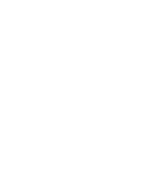
\includegraphics[width=110pt]{class_row_vector__coll__graph}
\end{center}
\end{figure}
\subsection*{Public Member Functions}
\begin{DoxyCompactItemize}
\item 
\hyperlink{class_row_vector_a2f27ef01198c0c996290f5d6d1680297}{RowVector} (int c)
\begin{DoxyCompactList}\small\item\em Creates a \hyperlink{class_row_vector}{RowVector} of the specified length. \item\end{DoxyCompactList}\item 
\hyperlink{class_row_vector_a6f0b27522b67138a7313c4a75750a7a6}{RowVector} (std::vector$<$ double $>$ \&a)
\begin{DoxyCompactList}\small\item\em Creates a \hyperlink{class_row_vector}{RowVector} from a vector of doubles. \item\end{DoxyCompactList}\item 
\hyperlink{class_row_vector_afdb9cc1d09c9dfaef6af93aec542f498}{RowVector} (double $\ast$a, int size)
\begin{DoxyCompactList}\small\item\em Creates a \hyperlink{class_row_vector}{RowVector} from an array of doubles, with the size of the array as the second argument. \item\end{DoxyCompactList}\item 
double \hyperlink{class_row_vector_a5c2dde299464fd200026db5515480275}{length} ()
\begin{DoxyCompactList}\small\item\em Calculates and returns the length of the vector. \item\end{DoxyCompactList}\item 
void \hyperlink{class_row_vector_aa04552c6bdfed758bc06815d8696b44c}{appendRow} ()
\begin{DoxyCompactList}\small\item\em This method is undefined for a \hyperlink{class_row_vector}{RowVector} since a \hyperlink{class_row_vector}{RowVector} can only have one row. \item\end{DoxyCompactList}\end{DoxyCompactItemize}


\subsection{Detailed Description}
The \hyperlink{class_row_vector}{RowVector} class, which inherits from the general \hyperlink{class_matrix}{Matrix} class. If you want to do vector-\/specific operations like get the length of the vector, use this class instead of the \hyperlink{class_matrix}{Matrix} class. 

\subsection{Constructor \& Destructor Documentation}
\hypertarget{class_row_vector_a2f27ef01198c0c996290f5d6d1680297}{
\index{RowVector@{RowVector}!RowVector@{RowVector}}
\index{RowVector@{RowVector}!RowVector@{RowVector}}
\subsubsection[{RowVector}]{\setlength{\rightskip}{0pt plus 5cm}RowVector::RowVector (int {\em c})\hspace{0.3cm}{\ttfamily  \mbox{[}inline, explicit\mbox{]}}}}
\label{class_row_vector_a2f27ef01198c0c996290f5d6d1680297}


Creates a \hyperlink{class_row_vector}{RowVector} of the specified length. 

\hypertarget{class_row_vector_a6f0b27522b67138a7313c4a75750a7a6}{
\index{RowVector@{RowVector}!RowVector@{RowVector}}
\index{RowVector@{RowVector}!RowVector@{RowVector}}
\subsubsection[{RowVector}]{\setlength{\rightskip}{0pt plus 5cm}RowVector::RowVector (std::vector$<$ double $>$ \& {\em a})}}
\label{class_row_vector_a6f0b27522b67138a7313c4a75750a7a6}


Creates a \hyperlink{class_row_vector}{RowVector} from a vector of doubles. 

\hypertarget{class_row_vector_afdb9cc1d09c9dfaef6af93aec542f498}{
\index{RowVector@{RowVector}!RowVector@{RowVector}}
\index{RowVector@{RowVector}!RowVector@{RowVector}}
\subsubsection[{RowVector}]{\setlength{\rightskip}{0pt plus 5cm}RowVector::RowVector (double $\ast$ {\em a}, \/  int {\em size})}}
\label{class_row_vector_afdb9cc1d09c9dfaef6af93aec542f498}


Creates a \hyperlink{class_row_vector}{RowVector} from an array of doubles, with the size of the array as the second argument. 



\subsection{Member Function Documentation}
\hypertarget{class_row_vector_aa04552c6bdfed758bc06815d8696b44c}{
\index{RowVector@{RowVector}!appendRow@{appendRow}}
\index{appendRow@{appendRow}!RowVector@{RowVector}}
\subsubsection[{appendRow}]{\setlength{\rightskip}{0pt plus 5cm}void RowVector::appendRow ()}}
\label{class_row_vector_aa04552c6bdfed758bc06815d8696b44c}


This method is undefined for a \hyperlink{class_row_vector}{RowVector} since a \hyperlink{class_row_vector}{RowVector} can only have one row. 

\hypertarget{class_row_vector_a5c2dde299464fd200026db5515480275}{
\index{RowVector@{RowVector}!length@{length}}
\index{length@{length}!RowVector@{RowVector}}
\subsubsection[{length}]{\setlength{\rightskip}{0pt plus 5cm}double RowVector::length ()}}
\label{class_row_vector_a5c2dde299464fd200026db5515480275}


Calculates and returns the length of the vector. 



The documentation for this class was generated from the following files:\begin{DoxyCompactItemize}
\item 
\hyperlink{_matrix_8h}{Matrix.h}\item 
\hyperlink{_matrix_8cpp}{Matrix.cpp}\end{DoxyCompactItemize}

\chapter{File Documentation}
\hypertarget{_matrix_8cpp}{
\section{Matrix.cpp File Reference}
\label{_matrix_8cpp}\index{Matrix.cpp@{Matrix.cpp}}
}
{\ttfamily \#include $<$iostream$>$}\par
{\ttfamily \#include $<$ctime$>$}\par
{\ttfamily \#include $<$cstdlib$>$}\par
{\ttfamily \#include $<$vector$>$}\par
{\ttfamily \#include $<$cassert$>$}\par
{\ttfamily \#include $<$cmath$>$}\par
{\ttfamily \#include \char`\"{}Matrix.h\char`\"{}}\par
{\ttfamily \#include \char`\"{}Matrix.h\char`\"{}}\par
{\ttfamily \#include \char`\"{}boost/tuple/tuple.hpp\char`\"{}}\par
Include dependency graph for Matrix.cpp:\nopagebreak
\begin{figure}[H]
\begin{center}
\leavevmode
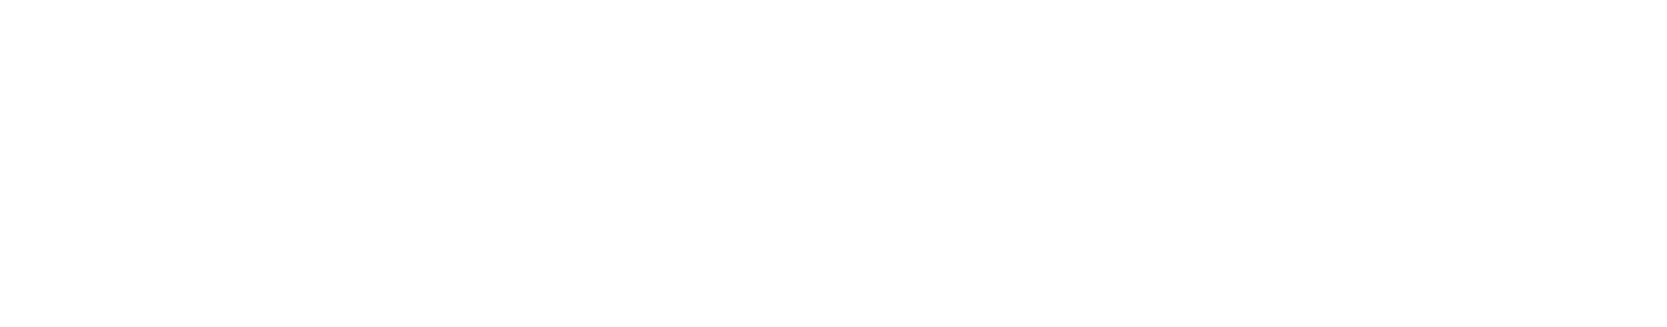
\includegraphics[width=276pt]{_matrix_8cpp__incl}
\end{center}
\end{figure}
This graph shows which files directly or indirectly include this file:\nopagebreak
\begin{figure}[H]
\begin{center}
\leavevmode
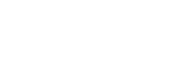
\includegraphics[width=63pt]{_matrix_8cpp__dep__incl}
\end{center}
\end{figure}
\subsection*{Functions}
\begin{DoxyCompactItemize}
\item 
\hyperlink{class_matrix}{Matrix} \& \hyperlink{_matrix_8cpp_aef0abd0dfab7b317c00f847ea7673842}{operator$\ast$} (\hyperlink{class_matrix}{Matrix} \&a, \hyperlink{class_matrix}{Matrix} \&b)
\begin{DoxyCompactList}\small\item\em Multiplies two matrices and returns the resulting \hyperlink{class_matrix}{Matrix} object. \item\end{DoxyCompactList}\item 
\hyperlink{class_matrix}{Matrix} \& \hyperlink{_matrix_8cpp_accade08db7bbcb399bf0f7f6fc0f7a38}{operator$\ast$} (double s, \hyperlink{class_matrix}{Matrix} \&a)
\begin{DoxyCompactList}\small\item\em Multiplies a \hyperlink{class_matrix}{Matrix} object by a scalar (double) and returns the resulting \hyperlink{class_matrix}{Matrix} object. \item\end{DoxyCompactList}\item 
\hyperlink{class_matrix}{Matrix} \& \hyperlink{_matrix_8cpp_aab165f42146537ca4960efd0e1c2975c}{operator$\ast$} (\hyperlink{class_matrix}{Matrix} \&a, double s)
\begin{DoxyCompactList}\small\item\em Multiplies a \hyperlink{class_matrix}{Matrix} object by a scalar (double) and returns the resulting \hyperlink{class_matrix}{Matrix} object. \item\end{DoxyCompactList}\item 
\hyperlink{class_matrix}{Matrix} \& \hyperlink{_matrix_8cpp_a3e861c2a1976635b49ded957b0fc1de1}{operator+} (\hyperlink{class_matrix}{Matrix} \&a, \hyperlink{class_matrix}{Matrix} \&b)
\begin{DoxyCompactList}\small\item\em Adds two \hyperlink{class_matrix}{Matrix} objects elementwise and returns the resulting \hyperlink{class_matrix}{Matrix} object. \item\end{DoxyCompactList}\item 
\hyperlink{class_matrix}{Matrix} \& \hyperlink{_matrix_8cpp_a3c8b27309dc425642323ec213fbce7aa}{operator-\/} (\hyperlink{class_matrix}{Matrix} \&a, \hyperlink{class_matrix}{Matrix} \&b)
\begin{DoxyCompactList}\small\item\em Subtracts the second matrix from the first matrix returns the resulting \hyperlink{class_matrix}{Matrix} object. \item\end{DoxyCompactList}\item 
ostream \& \hyperlink{_matrix_8cpp_ae88f31e57329a153343a5f1fb714c88f}{operator$<$$<$} (ostream \&s, \hyperlink{class_matrix}{Matrix} \&m)
\item 
bool \hyperlink{_matrix_8cpp_a521b4fbb24969f12c91690fdada71daa}{operator==} (\hyperlink{class_matrix}{Matrix} \&a, \hyperlink{class_matrix}{Matrix} \&b)
\begin{DoxyCompactList}\small\item\em Tests if two \hyperlink{class_matrix}{Matrix} objects are equivalent. \item\end{DoxyCompactList}\end{DoxyCompactItemize}


\subsection{Function Documentation}
\hypertarget{_matrix_8cpp_aab165f42146537ca4960efd0e1c2975c}{
\index{Matrix.cpp@{Matrix.cpp}!operator$\ast$@{operator$\ast$}}
\index{operator$\ast$@{operator$\ast$}!Matrix.cpp@{Matrix.cpp}}
\subsubsection[{operator$\ast$}]{\setlength{\rightskip}{0pt plus 5cm}{\bf Matrix} \& operator$\ast$ ({\bf Matrix} \& {\em a}, \/  double {\em s})}}
\label{_matrix_8cpp_aab165f42146537ca4960efd0e1c2975c}


Multiplies a \hyperlink{class_matrix}{Matrix} object by a scalar (double) and returns the resulting \hyperlink{class_matrix}{Matrix} object. 

\hypertarget{_matrix_8cpp_accade08db7bbcb399bf0f7f6fc0f7a38}{
\index{Matrix.cpp@{Matrix.cpp}!operator$\ast$@{operator$\ast$}}
\index{operator$\ast$@{operator$\ast$}!Matrix.cpp@{Matrix.cpp}}
\subsubsection[{operator$\ast$}]{\setlength{\rightskip}{0pt plus 5cm}{\bf Matrix} \& operator$\ast$ (double {\em s}, \/  {\bf Matrix} \& {\em a})}}
\label{_matrix_8cpp_accade08db7bbcb399bf0f7f6fc0f7a38}


Multiplies a \hyperlink{class_matrix}{Matrix} object by a scalar (double) and returns the resulting \hyperlink{class_matrix}{Matrix} object. 

\hypertarget{_matrix_8cpp_aef0abd0dfab7b317c00f847ea7673842}{
\index{Matrix.cpp@{Matrix.cpp}!operator$\ast$@{operator$\ast$}}
\index{operator$\ast$@{operator$\ast$}!Matrix.cpp@{Matrix.cpp}}
\subsubsection[{operator$\ast$}]{\setlength{\rightskip}{0pt plus 5cm}{\bf Matrix} \& operator$\ast$ ({\bf Matrix} \& {\em a}, \/  {\bf Matrix} \& {\em b})}}
\label{_matrix_8cpp_aef0abd0dfab7b317c00f847ea7673842}


Multiplies two matrices and returns the resulting \hyperlink{class_matrix}{Matrix} object. 

\hypertarget{_matrix_8cpp_a3e861c2a1976635b49ded957b0fc1de1}{
\index{Matrix.cpp@{Matrix.cpp}!operator+@{operator+}}
\index{operator+@{operator+}!Matrix.cpp@{Matrix.cpp}}
\subsubsection[{operator+}]{\setlength{\rightskip}{0pt plus 5cm}{\bf Matrix} \& operator+ ({\bf Matrix} \& {\em a}, \/  {\bf Matrix} \& {\em b})}}
\label{_matrix_8cpp_a3e861c2a1976635b49ded957b0fc1de1}


Adds two \hyperlink{class_matrix}{Matrix} objects elementwise and returns the resulting \hyperlink{class_matrix}{Matrix} object. 

\hypertarget{_matrix_8cpp_a3c8b27309dc425642323ec213fbce7aa}{
\index{Matrix.cpp@{Matrix.cpp}!operator-\/@{operator-\/}}
\index{operator-\/@{operator-\/}!Matrix.cpp@{Matrix.cpp}}
\subsubsection[{operator-\/}]{\setlength{\rightskip}{0pt plus 5cm}{\bf Matrix} \& operator-\/ ({\bf Matrix} \& {\em a}, \/  {\bf Matrix} \& {\em b})}}
\label{_matrix_8cpp_a3c8b27309dc425642323ec213fbce7aa}


Subtracts the second matrix from the first matrix returns the resulting \hyperlink{class_matrix}{Matrix} object. 

\hypertarget{_matrix_8cpp_ae88f31e57329a153343a5f1fb714c88f}{
\index{Matrix.cpp@{Matrix.cpp}!operator$<$$<$@{operator$<$$<$}}
\index{operator$<$$<$@{operator$<$$<$}!Matrix.cpp@{Matrix.cpp}}
\subsubsection[{operator$<$$<$}]{\setlength{\rightskip}{0pt plus 5cm}ostream\& operator$<$$<$ (ostream \& {\em s}, \/  {\bf Matrix} \& {\em m})}}
\label{_matrix_8cpp_ae88f31e57329a153343a5f1fb714c88f}
\hypertarget{_matrix_8cpp_a521b4fbb24969f12c91690fdada71daa}{
\index{Matrix.cpp@{Matrix.cpp}!operator==@{operator==}}
\index{operator==@{operator==}!Matrix.cpp@{Matrix.cpp}}
\subsubsection[{operator==}]{\setlength{\rightskip}{0pt plus 5cm}bool operator== ({\bf Matrix} \& {\em a}, \/  {\bf Matrix} \& {\em b})}}
\label{_matrix_8cpp_a521b4fbb24969f12c91690fdada71daa}


Tests if two \hyperlink{class_matrix}{Matrix} objects are equivalent. 


\hypertarget{_matrix_8h}{
\section{Matrix.h File Reference}
\label{_matrix_8h}\index{Matrix.h@{Matrix.h}}
}


This file contains the declarations of the basic Linear Algebra classes and some methods that operate on them.  


{\ttfamily \#include $<$iostream$>$}\par
{\ttfamily \#include $<$vector$>$}\par
Include dependency graph for Matrix.h:\nopagebreak
\begin{figure}[H]
\begin{center}
\leavevmode
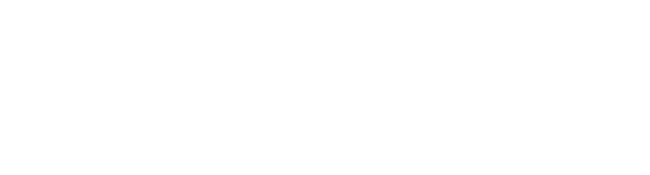
\includegraphics[width=81pt]{_matrix_8h__incl}
\end{center}
\end{figure}
This graph shows which files directly or indirectly include this file:\nopagebreak
\begin{figure}[H]
\begin{center}
\leavevmode
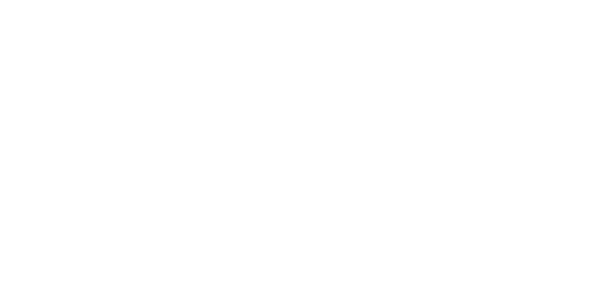
\includegraphics[width=160pt]{_matrix_8h__dep__incl}
\end{center}
\end{figure}
\subsection*{Classes}
\begin{DoxyCompactItemize}
\item 
class \hyperlink{class_matrix}{Matrix}
\begin{DoxyCompactList}\small\item\em The general \hyperlink{class_matrix}{Matrix} class. \item\end{DoxyCompactList}\item 
class \hyperlink{class_row_vector}{RowVector}
\begin{DoxyCompactList}\small\item\em The \hyperlink{class_row_vector}{RowVector} class, which inherits from the general \hyperlink{class_matrix}{Matrix} class. \item\end{DoxyCompactList}\item 
class \hyperlink{class_column_vector}{ColumnVector}
\begin{DoxyCompactList}\small\item\em The \hyperlink{class_column_vector}{ColumnVector} class, which inherits from the general \hyperlink{class_matrix}{Matrix} class. \item\end{DoxyCompactList}\end{DoxyCompactItemize}
\subsection*{Functions}
\begin{DoxyCompactItemize}
\item 
\hyperlink{class_matrix}{Matrix} \& \hyperlink{_matrix_8h_a583d1589aee3559d4442488c512046a5}{operator$\ast$} (\hyperlink{class_matrix}{Matrix} \&a, \hyperlink{class_matrix}{Matrix} \&b)
\begin{DoxyCompactList}\small\item\em Multiplies two matrices and returns the resulting \hyperlink{class_matrix}{Matrix} object. \item\end{DoxyCompactList}\item 
\hyperlink{class_matrix}{Matrix} \& \hyperlink{_matrix_8h_ac7712e631a367916e502bba3761b63de}{operator$\ast$} (double s, \hyperlink{class_matrix}{Matrix} \&a)
\begin{DoxyCompactList}\small\item\em Multiplies a \hyperlink{class_matrix}{Matrix} object by a scalar (double) and returns the resulting \hyperlink{class_matrix}{Matrix} object. \item\end{DoxyCompactList}\item 
\hyperlink{class_matrix}{Matrix} \& \hyperlink{_matrix_8h_ad6a8417fcb147d2bbecbe674572d57b9}{operator$\ast$} (\hyperlink{class_matrix}{Matrix} \&a, double s)
\begin{DoxyCompactList}\small\item\em Multiplies a \hyperlink{class_matrix}{Matrix} object by a scalar (double) and returns the resulting \hyperlink{class_matrix}{Matrix} object. \item\end{DoxyCompactList}\item 
\hyperlink{class_matrix}{Matrix} \& \hyperlink{_matrix_8h_afdfd38437764622830248868384327b9}{operator+} (\hyperlink{class_matrix}{Matrix} \&a, \hyperlink{class_matrix}{Matrix} \&b)
\begin{DoxyCompactList}\small\item\em Adds two \hyperlink{class_matrix}{Matrix} objects elementwise and returns the resulting \hyperlink{class_matrix}{Matrix} object. \item\end{DoxyCompactList}\item 
\hyperlink{class_matrix}{Matrix} \& \hyperlink{_matrix_8h_ac9e409817c609f095d0fe666b1093f0e}{operator-\/} (\hyperlink{class_matrix}{Matrix} \&a, \hyperlink{class_matrix}{Matrix} \&b)
\begin{DoxyCompactList}\small\item\em Subtracts the second matrix from the first matrix returns the resulting \hyperlink{class_matrix}{Matrix} object. \item\end{DoxyCompactList}\item 
std::ostream \& \hyperlink{_matrix_8h_aa4a618cf39cf99ebadd2b230fbbacfd5}{operator$<$$<$} (std::ostream \&s, \hyperlink{class_matrix}{Matrix} \&m)
\begin{DoxyCompactList}\small\item\em Prints out a \hyperlink{class_matrix}{Matrix} object. \item\end{DoxyCompactList}\item 
bool \hyperlink{_matrix_8h_a521b4fbb24969f12c91690fdada71daa}{operator==} (\hyperlink{class_matrix}{Matrix} \&a, \hyperlink{class_matrix}{Matrix} \&b)
\begin{DoxyCompactList}\small\item\em Tests if two \hyperlink{class_matrix}{Matrix} objects are equivalent. \item\end{DoxyCompactList}\end{DoxyCompactItemize}


\subsection{Detailed Description}
This file contains the declarations of the basic Linear Algebra classes and some methods that operate on them. 

\subsection{Function Documentation}
\hypertarget{_matrix_8h_ad6a8417fcb147d2bbecbe674572d57b9}{
\index{Matrix.h@{Matrix.h}!operator$\ast$@{operator$\ast$}}
\index{operator$\ast$@{operator$\ast$}!Matrix.h@{Matrix.h}}
\subsubsection[{operator$\ast$}]{\setlength{\rightskip}{0pt plus 5cm}{\bf Matrix}\& operator$\ast$ ({\bf Matrix} \& {\em a}, \/  double {\em s})}}
\label{_matrix_8h_ad6a8417fcb147d2bbecbe674572d57b9}


Multiplies a \hyperlink{class_matrix}{Matrix} object by a scalar (double) and returns the resulting \hyperlink{class_matrix}{Matrix} object. 

\hypertarget{_matrix_8h_ac7712e631a367916e502bba3761b63de}{
\index{Matrix.h@{Matrix.h}!operator$\ast$@{operator$\ast$}}
\index{operator$\ast$@{operator$\ast$}!Matrix.h@{Matrix.h}}
\subsubsection[{operator$\ast$}]{\setlength{\rightskip}{0pt plus 5cm}{\bf Matrix}\& operator$\ast$ (double {\em s}, \/  {\bf Matrix} \& {\em a})}}
\label{_matrix_8h_ac7712e631a367916e502bba3761b63de}


Multiplies a \hyperlink{class_matrix}{Matrix} object by a scalar (double) and returns the resulting \hyperlink{class_matrix}{Matrix} object. 

\hypertarget{_matrix_8h_a583d1589aee3559d4442488c512046a5}{
\index{Matrix.h@{Matrix.h}!operator$\ast$@{operator$\ast$}}
\index{operator$\ast$@{operator$\ast$}!Matrix.h@{Matrix.h}}
\subsubsection[{operator$\ast$}]{\setlength{\rightskip}{0pt plus 5cm}{\bf Matrix}\& operator$\ast$ ({\bf Matrix} \& {\em a}, \/  {\bf Matrix} \& {\em b})}}
\label{_matrix_8h_a583d1589aee3559d4442488c512046a5}


Multiplies two matrices and returns the resulting \hyperlink{class_matrix}{Matrix} object. 

\hypertarget{_matrix_8h_afdfd38437764622830248868384327b9}{
\index{Matrix.h@{Matrix.h}!operator+@{operator+}}
\index{operator+@{operator+}!Matrix.h@{Matrix.h}}
\subsubsection[{operator+}]{\setlength{\rightskip}{0pt plus 5cm}{\bf Matrix}\& operator+ ({\bf Matrix} \& {\em a}, \/  {\bf Matrix} \& {\em b})}}
\label{_matrix_8h_afdfd38437764622830248868384327b9}


Adds two \hyperlink{class_matrix}{Matrix} objects elementwise and returns the resulting \hyperlink{class_matrix}{Matrix} object. 

\hypertarget{_matrix_8h_ac9e409817c609f095d0fe666b1093f0e}{
\index{Matrix.h@{Matrix.h}!operator-\/@{operator-\/}}
\index{operator-\/@{operator-\/}!Matrix.h@{Matrix.h}}
\subsubsection[{operator-\/}]{\setlength{\rightskip}{0pt plus 5cm}{\bf Matrix}\& operator-\/ ({\bf Matrix} \& {\em a}, \/  {\bf Matrix} \& {\em b})}}
\label{_matrix_8h_ac9e409817c609f095d0fe666b1093f0e}


Subtracts the second matrix from the first matrix returns the resulting \hyperlink{class_matrix}{Matrix} object. 

\hypertarget{_matrix_8h_aa4a618cf39cf99ebadd2b230fbbacfd5}{
\index{Matrix.h@{Matrix.h}!operator$<$$<$@{operator$<$$<$}}
\index{operator$<$$<$@{operator$<$$<$}!Matrix.h@{Matrix.h}}
\subsubsection[{operator$<$$<$}]{\setlength{\rightskip}{0pt plus 5cm}std::ostream \& operator$<$$<$ (std::ostream \& {\em s}, \/  {\bf Matrix} \& {\em m})}}
\label{_matrix_8h_aa4a618cf39cf99ebadd2b230fbbacfd5}


Prints out a \hyperlink{class_matrix}{Matrix} object. 

\hypertarget{_matrix_8h_a521b4fbb24969f12c91690fdada71daa}{
\index{Matrix.h@{Matrix.h}!operator==@{operator==}}
\index{operator==@{operator==}!Matrix.h@{Matrix.h}}
\subsubsection[{operator==}]{\setlength{\rightskip}{0pt plus 5cm}bool operator== ({\bf Matrix} \& {\em a}, \/  {\bf Matrix} \& {\em b})}}
\label{_matrix_8h_a521b4fbb24969f12c91690fdada71daa}


Tests if two \hyperlink{class_matrix}{Matrix} objects are equivalent. 


\hypertarget{_matrix_functions_8cpp}{
\section{MatrixFunctions.cpp File Reference}
\label{_matrix_functions_8cpp}\index{MatrixFunctions.cpp@{MatrixFunctions.cpp}}
}
{\ttfamily \#include $<$memory$>$}\par
{\ttfamily \#include \char`\"{}MatrixFunctions.h\char`\"{}}\par
{\ttfamily \#include \char`\"{}Matrix.h\char`\"{}}\par
{\ttfamily \#include $<$boost/tuple/tuple.hpp$>$}\par
{\ttfamily \#include $<$boost/shared\_\-ptr.hpp$>$}\par
Include dependency graph for MatrixFunctions.cpp:\nopagebreak
\begin{figure}[H]
\begin{center}
\leavevmode
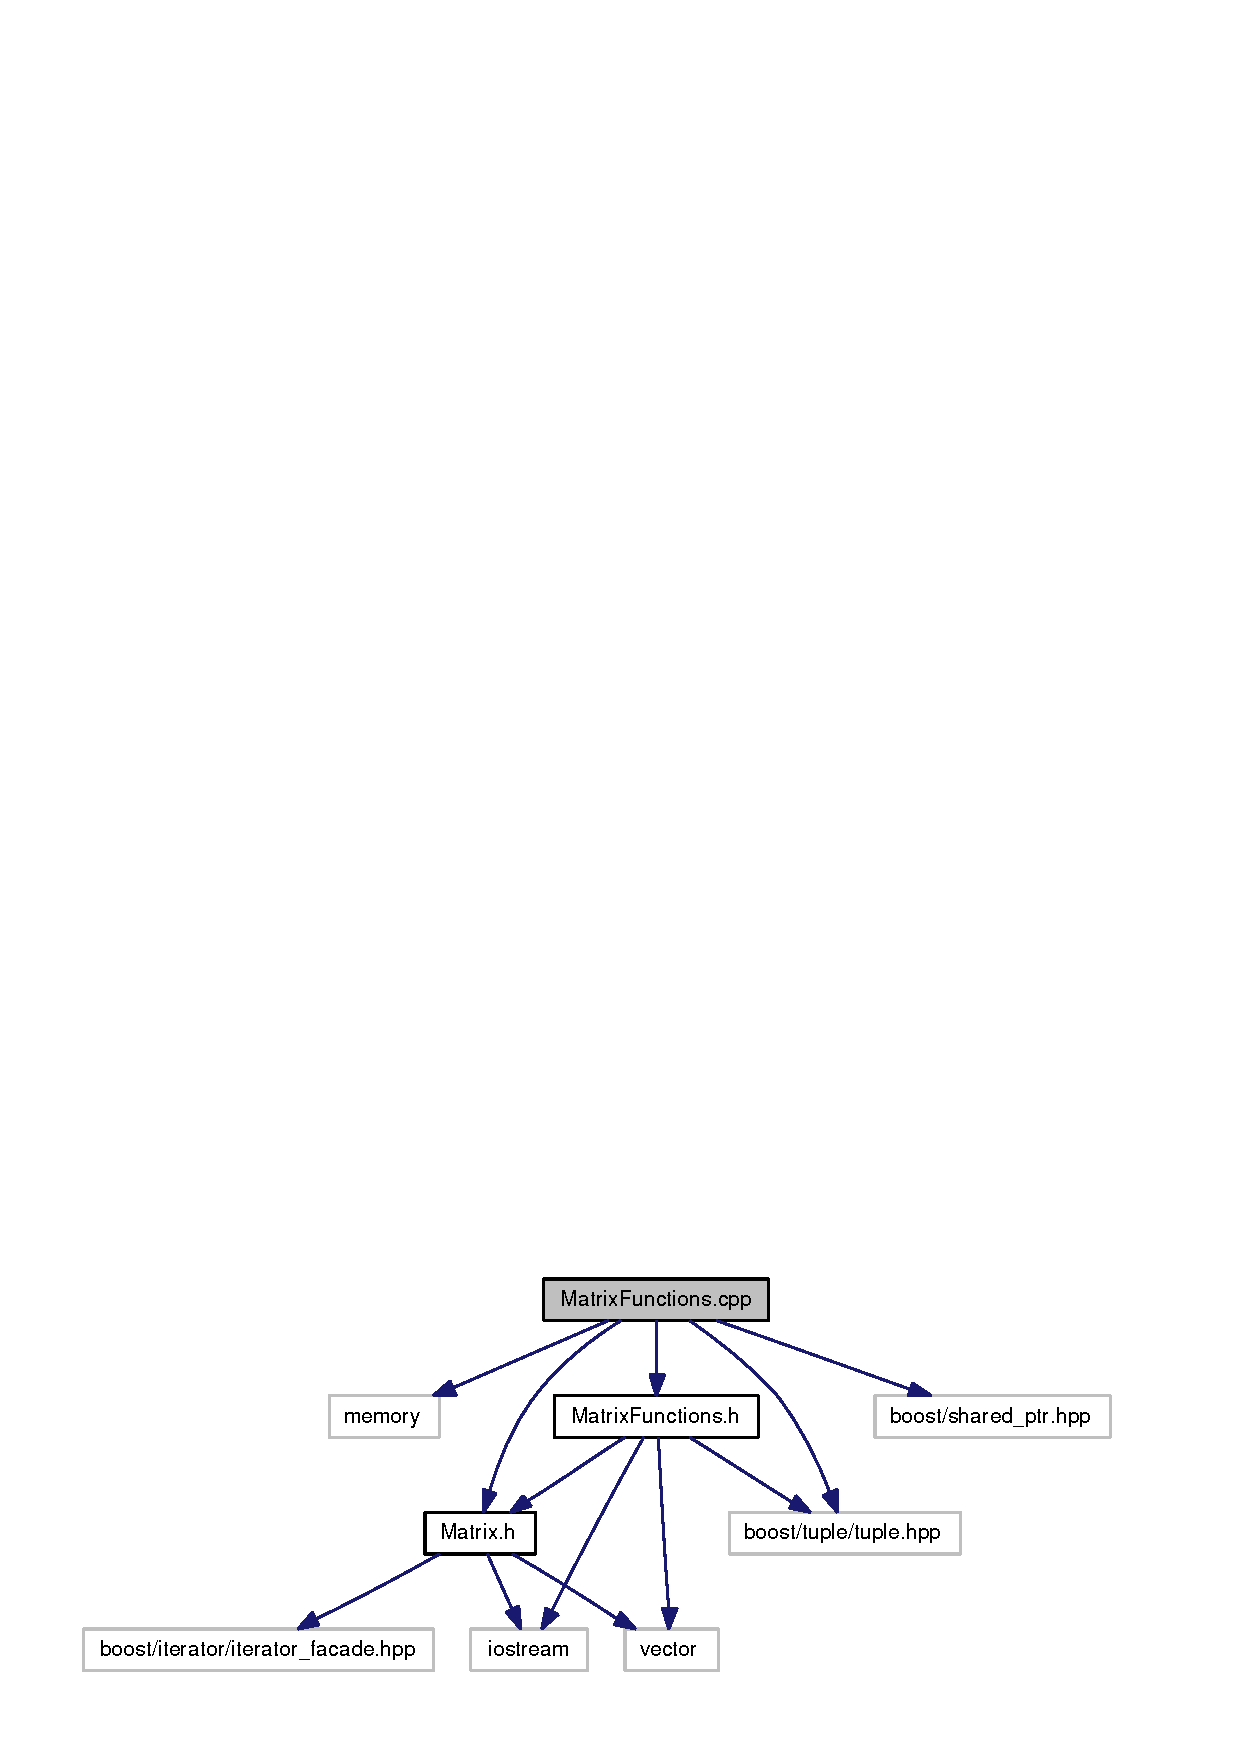
\includegraphics[width=268pt]{_matrix_functions_8cpp__incl}
\end{center}
\end{figure}
\subsection*{Functions}
\begin{DoxyCompactItemize}
\item 
int \hyperlink{_matrix_functions_8cpp_aa7678f1d5dfe64cad1897e1a78da2c10}{findNonZero} (\hyperlink{class_matrix}{Matrix} \&m, int col)
\begin{DoxyCompactList}\small\item\em Given a \hyperlink{class_matrix}{Matrix} and a column number, this functions returns the index of the first row which has a non-\/zero value in that column. \item\end{DoxyCompactList}\item 
\hyperlink{class_matrix}{Matrix} \hyperlink{_matrix_functions_8cpp_aec58045132edaf43914a134b4eb2697f}{gaussJordan} (\hyperlink{class_matrix}{Matrix} \&A, \hyperlink{class_matrix}{Matrix} \&b)
\begin{DoxyCompactList}\small\item\em Given two matrices A and b, solves the linear system of equations assuming the form Ax = b. \item\end{DoxyCompactList}\item 
\hyperlink{class_matrix}{Matrix} \hyperlink{_matrix_functions_8cpp_a5ab64c0532a96fd250bf278423b326cf}{gaussianElimination} (\hyperlink{class_matrix}{Matrix} \&A, \hyperlink{class_matrix}{Matrix} \&b)
\begin{DoxyCompactList}\small\item\em Given two matrices A and b, solves the linear system of equations assuming the form Ax = b. \item\end{DoxyCompactList}\item 
boost::tuple$<$ \hyperlink{class_matrix}{Matrix}, \hyperlink{class_matrix}{Matrix}, \hyperlink{class_matrix}{Matrix} $>$ \hyperlink{_matrix_functions_8cpp_a4211ea2b9a4462e11be36b7ab09ebf5a}{LUPDecompose} (\hyperlink{class_matrix}{Matrix} A)
\begin{DoxyCompactList}\small\item\em Given a matrix, returns it's LUP decomposition. \item\end{DoxyCompactList}\end{DoxyCompactItemize}


\subsection{Function Documentation}
\hypertarget{_matrix_functions_8cpp_aa7678f1d5dfe64cad1897e1a78da2c10}{
\index{MatrixFunctions.cpp@{MatrixFunctions.cpp}!findNonZero@{findNonZero}}
\index{findNonZero@{findNonZero}!MatrixFunctions.cpp@{MatrixFunctions.cpp}}
\subsubsection[{findNonZero}]{\setlength{\rightskip}{0pt plus 5cm}int findNonZero ({\bf Matrix} \& {\em m}, \/  int {\em col})}}
\label{_matrix_functions_8cpp_aa7678f1d5dfe64cad1897e1a78da2c10}


Given a \hyperlink{class_matrix}{Matrix} and a column number, this functions returns the index of the first row which has a non-\/zero value in that column. 

If all rows have zeroes, it returns -\/1. This function is used by both gaussJordan and gaussianElimination. \hypertarget{_matrix_functions_8cpp_a5ab64c0532a96fd250bf278423b326cf}{
\index{MatrixFunctions.cpp@{MatrixFunctions.cpp}!gaussianElimination@{gaussianElimination}}
\index{gaussianElimination@{gaussianElimination}!MatrixFunctions.cpp@{MatrixFunctions.cpp}}
\subsubsection[{gaussianElimination}]{\setlength{\rightskip}{0pt plus 5cm}{\bf Matrix} \& gaussianElimination ({\bf Matrix} \& {\em A}, \/  {\bf Matrix} \& {\em b})}}
\label{_matrix_functions_8cpp_a5ab64c0532a96fd250bf278423b326cf}


Given two matrices A and b, solves the linear system of equations assuming the form Ax = b. 

Uses Gaussian Elimination with backsubstitution. Returns a \hyperlink{class_matrix}{Matrix} object containing the solution. \hypertarget{_matrix_functions_8cpp_aec58045132edaf43914a134b4eb2697f}{
\index{MatrixFunctions.cpp@{MatrixFunctions.cpp}!gaussJordan@{gaussJordan}}
\index{gaussJordan@{gaussJordan}!MatrixFunctions.cpp@{MatrixFunctions.cpp}}
\subsubsection[{gaussJordan}]{\setlength{\rightskip}{0pt plus 5cm}{\bf Matrix} \& gaussJordan ({\bf Matrix} \& {\em A}, \/  {\bf Matrix} \& {\em b})}}
\label{_matrix_functions_8cpp_aec58045132edaf43914a134b4eb2697f}


Given two matrices A and b, solves the linear system of equations assuming the form Ax = b. 

Uses Gauss-\/Jordan. Returns a \hyperlink{class_matrix}{Matrix} object containing the solution. \hypertarget{_matrix_functions_8cpp_a4211ea2b9a4462e11be36b7ab09ebf5a}{
\index{MatrixFunctions.cpp@{MatrixFunctions.cpp}!LUPDecompose@{LUPDecompose}}
\index{LUPDecompose@{LUPDecompose}!MatrixFunctions.cpp@{MatrixFunctions.cpp}}
\subsubsection[{LUPDecompose}]{\setlength{\rightskip}{0pt plus 5cm}boost::tuple$<$ {\bf Matrix}, {\bf Matrix}, {\bf Matrix} $>$ LUPDecompose ({\bf Matrix} {\em A})}}
\label{_matrix_functions_8cpp_a4211ea2b9a4462e11be36b7ab09ebf5a}


Given a matrix, returns it's LUP decomposition. 

Three matrices L, U and P are returned as a boost tuple. Example usage: 
\begin{DoxyCode}
    #include "boost/tuple/tuple.hpp"

    // create a new matrix
    Matrix A(3,3);
    A.populateRandom();
  
    // get its decomposition
    boost::tuple<Matrix,Matrix,Matrix> lu = LUPDecompose(A);
    Matrix L = lu.get<0>();
    Matrix U = lu.get<1>();
    Matrix P = lu.get<2>();
    
    // print out matrices
    cout << L << endl;
    cout << U << endl;
    cout << P << endl;
\end{DoxyCode}
 
\hypertarget{_matrix_functions_8h}{
\section{MatrixFunctions.h File Reference}
\label{_matrix_functions_8h}\index{MatrixFunctions.h@{MatrixFunctions.h}}
}


This file contains the declarations of the basic Linear Algebra classes and some methods that operate on them.  


{\ttfamily \#include $<$iostream$>$}\par
{\ttfamily \#include $<$vector$>$}\par
{\ttfamily \#include \char`\"{}Matrix.h\char`\"{}}\par
{\ttfamily \#include \char`\"{}boost/tuple/tuple.hpp\char`\"{}}\par
Include dependency graph for MatrixFunctions.h:\nopagebreak
\begin{figure}[H]
\begin{center}
\leavevmode
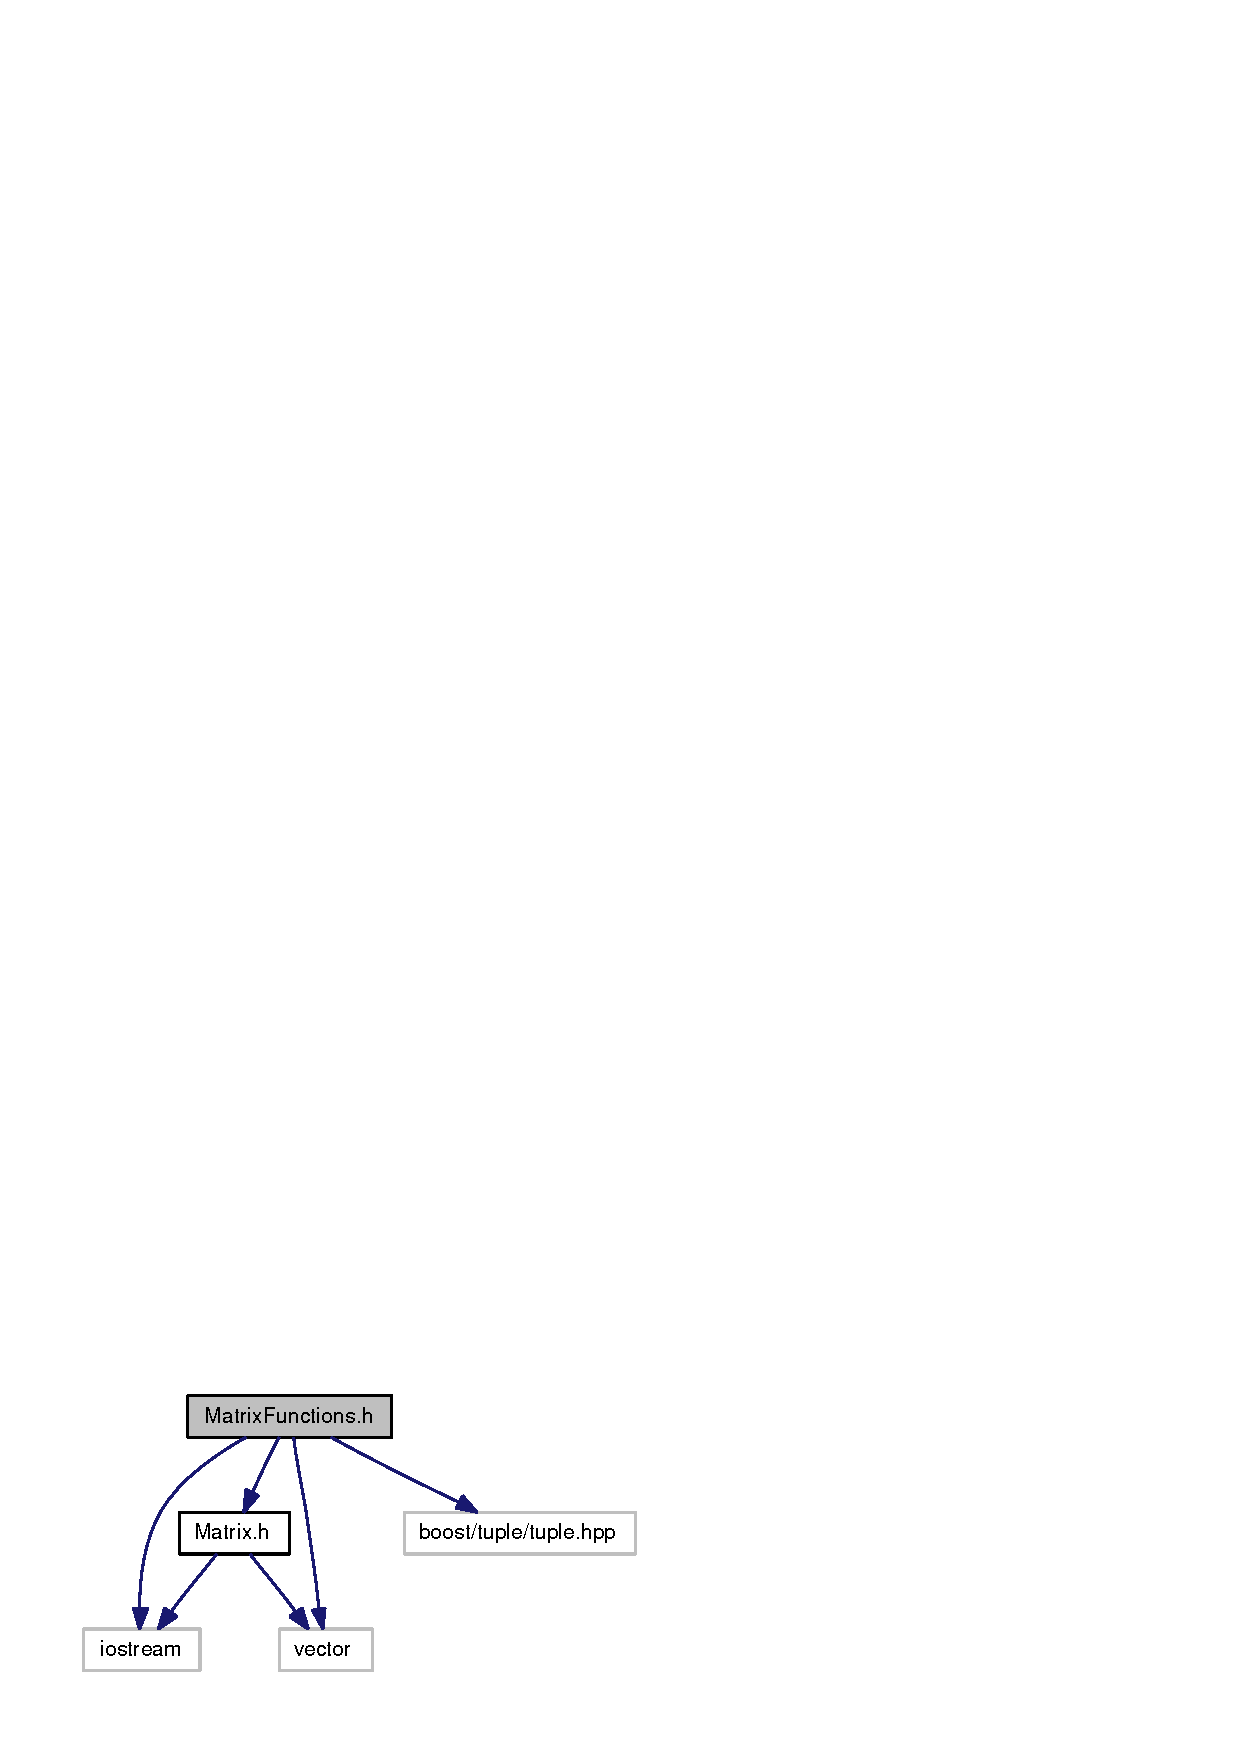
\includegraphics[width=154pt]{_matrix_functions_8h__incl}
\end{center}
\end{figure}
This graph shows which files directly or indirectly include this file:\nopagebreak
\begin{figure}[H]
\begin{center}
\leavevmode
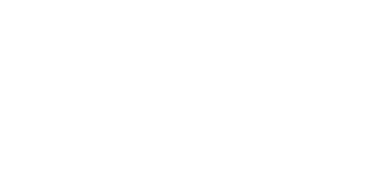
\includegraphics[width=111pt]{_matrix_functions_8h__dep__incl}
\end{center}
\end{figure}
\subsection*{Functions}
\begin{DoxyCompactItemize}
\item 
int \hyperlink{_matrix_functions_8h_aa7678f1d5dfe64cad1897e1a78da2c10}{findNonZero} (\hyperlink{class_matrix}{Matrix} \&m, int col)
\begin{DoxyCompactList}\small\item\em Given a \hyperlink{class_matrix}{Matrix} and a column number, this functions returns the index of the first row which has a non-\/zero value in that column. \item\end{DoxyCompactList}\item 
\hyperlink{class_matrix}{Matrix} \& \hyperlink{_matrix_functions_8h_a77b7bbc23b94764daf1def2756ed78a2}{gaussJordan} (\hyperlink{class_matrix}{Matrix} \&A, \hyperlink{class_matrix}{Matrix} \&b)
\begin{DoxyCompactList}\small\item\em Given two matrices A and b, solves the linear system of equations assuming the form Ax = b. \item\end{DoxyCompactList}\item 
\hyperlink{class_matrix}{Matrix} \& \hyperlink{_matrix_functions_8h_ae3f5418ded795e1220e7caac7771494b}{gaussianElimination} (\hyperlink{class_matrix}{Matrix} \&A, \hyperlink{class_matrix}{Matrix} \&b)
\begin{DoxyCompactList}\small\item\em Given two matrices A and b, solves the linear system of equations assuming the form Ax = b. \item\end{DoxyCompactList}\item 
boost::tuple$<$ \hyperlink{class_matrix}{Matrix}, \hyperlink{class_matrix}{Matrix}, \hyperlink{class_matrix}{Matrix} $>$ \hyperlink{_matrix_functions_8h_a3a79c07a22dd5e176404f713b54e5dfc}{LUPDecompose} (\hyperlink{class_matrix}{Matrix} A)
\begin{DoxyCompactList}\small\item\em Given a matrix, returns it's LUP decomposition. \item\end{DoxyCompactList}\end{DoxyCompactItemize}


\subsection{Detailed Description}
This file contains the declarations of the basic Linear Algebra classes and some methods that operate on them. 

\subsection{Function Documentation}
\hypertarget{_matrix_functions_8h_aa7678f1d5dfe64cad1897e1a78da2c10}{
\index{MatrixFunctions.h@{MatrixFunctions.h}!findNonZero@{findNonZero}}
\index{findNonZero@{findNonZero}!MatrixFunctions.h@{MatrixFunctions.h}}
\subsubsection[{findNonZero}]{\setlength{\rightskip}{0pt plus 5cm}int findNonZero ({\bf Matrix} \& {\em m}, \/  int {\em col})}}
\label{_matrix_functions_8h_aa7678f1d5dfe64cad1897e1a78da2c10}


Given a \hyperlink{class_matrix}{Matrix} and a column number, this functions returns the index of the first row which has a non-\/zero value in that column. 

If all rows have zeroes, it returns -\/1. This function is used by both gaussJordan and gaussianElimination. \hypertarget{_matrix_functions_8h_ae3f5418ded795e1220e7caac7771494b}{
\index{MatrixFunctions.h@{MatrixFunctions.h}!gaussianElimination@{gaussianElimination}}
\index{gaussianElimination@{gaussianElimination}!MatrixFunctions.h@{MatrixFunctions.h}}
\subsubsection[{gaussianElimination}]{\setlength{\rightskip}{0pt plus 5cm}{\bf Matrix}\& gaussianElimination ({\bf Matrix} \& {\em A}, \/  {\bf Matrix} \& {\em b})}}
\label{_matrix_functions_8h_ae3f5418ded795e1220e7caac7771494b}


Given two matrices A and b, solves the linear system of equations assuming the form Ax = b. 

Uses Gaussian Elimination with backsubstitution. Returns a \hyperlink{class_matrix}{Matrix} object containing the solution. \hypertarget{_matrix_functions_8h_a77b7bbc23b94764daf1def2756ed78a2}{
\index{MatrixFunctions.h@{MatrixFunctions.h}!gaussJordan@{gaussJordan}}
\index{gaussJordan@{gaussJordan}!MatrixFunctions.h@{MatrixFunctions.h}}
\subsubsection[{gaussJordan}]{\setlength{\rightskip}{0pt plus 5cm}{\bf Matrix}\& gaussJordan ({\bf Matrix} \& {\em A}, \/  {\bf Matrix} \& {\em b})}}
\label{_matrix_functions_8h_a77b7bbc23b94764daf1def2756ed78a2}


Given two matrices A and b, solves the linear system of equations assuming the form Ax = b. 

Uses Gauss-\/Jordan. Returns a \hyperlink{class_matrix}{Matrix} object containing the solution. \hypertarget{_matrix_functions_8h_a3a79c07a22dd5e176404f713b54e5dfc}{
\index{MatrixFunctions.h@{MatrixFunctions.h}!LUPDecompose@{LUPDecompose}}
\index{LUPDecompose@{LUPDecompose}!MatrixFunctions.h@{MatrixFunctions.h}}
\subsubsection[{LUPDecompose}]{\setlength{\rightskip}{0pt plus 5cm}boost::tuple$<${\bf Matrix}, {\bf Matrix}, {\bf Matrix}$>$ LUPDecompose ({\bf Matrix} {\em A})}}
\label{_matrix_functions_8h_a3a79c07a22dd5e176404f713b54e5dfc}


Given a matrix, returns it's LUP decomposition. 

Three matrices L, U and P are returned as a boost tuple. Example usage: 
\begin{DoxyCode}
    #include "boost/tuple/tuple.hpp"

    // create a new matrix
    Matrix A(3,3);
    A.populateRandom();
  
    // get its decomposition
    boost::tuple<Matrix,Matrix,Matrix> lu = LUPDecompose(A);
    Matrix L = lu.get<0>();
    Matrix U = lu.get<1>();
    Matrix P = lu.get<2>();
    
    // print out matrices
    cout << L << endl;
    cout << U << endl;
    cout << P << endl;
\end{DoxyCode}
 
\hypertarget{test_8cpp}{
\section{test.cpp File Reference}
\label{test_8cpp}\index{test.cpp@{test.cpp}}
}
{\ttfamily \#include $<$iostream$>$}\par
{\ttfamily \#include \char`\"{}Matrix.h\char`\"{}}\par
{\ttfamily \#include \char`\"{}MatrixFunctions.h\char`\"{}}\par
{\ttfamily \#include \char`\"{}boost/tuple/tuple.hpp\char`\"{}}\par
{\ttfamily \#include $<$vector$>$}\par
{\ttfamily \#include $<$algorithm$>$}\par
{\ttfamily \#include $<$numeric$>$}\par
Include dependency graph for test.cpp:\nopagebreak
\begin{figure}[H]
\begin{center}
\leavevmode
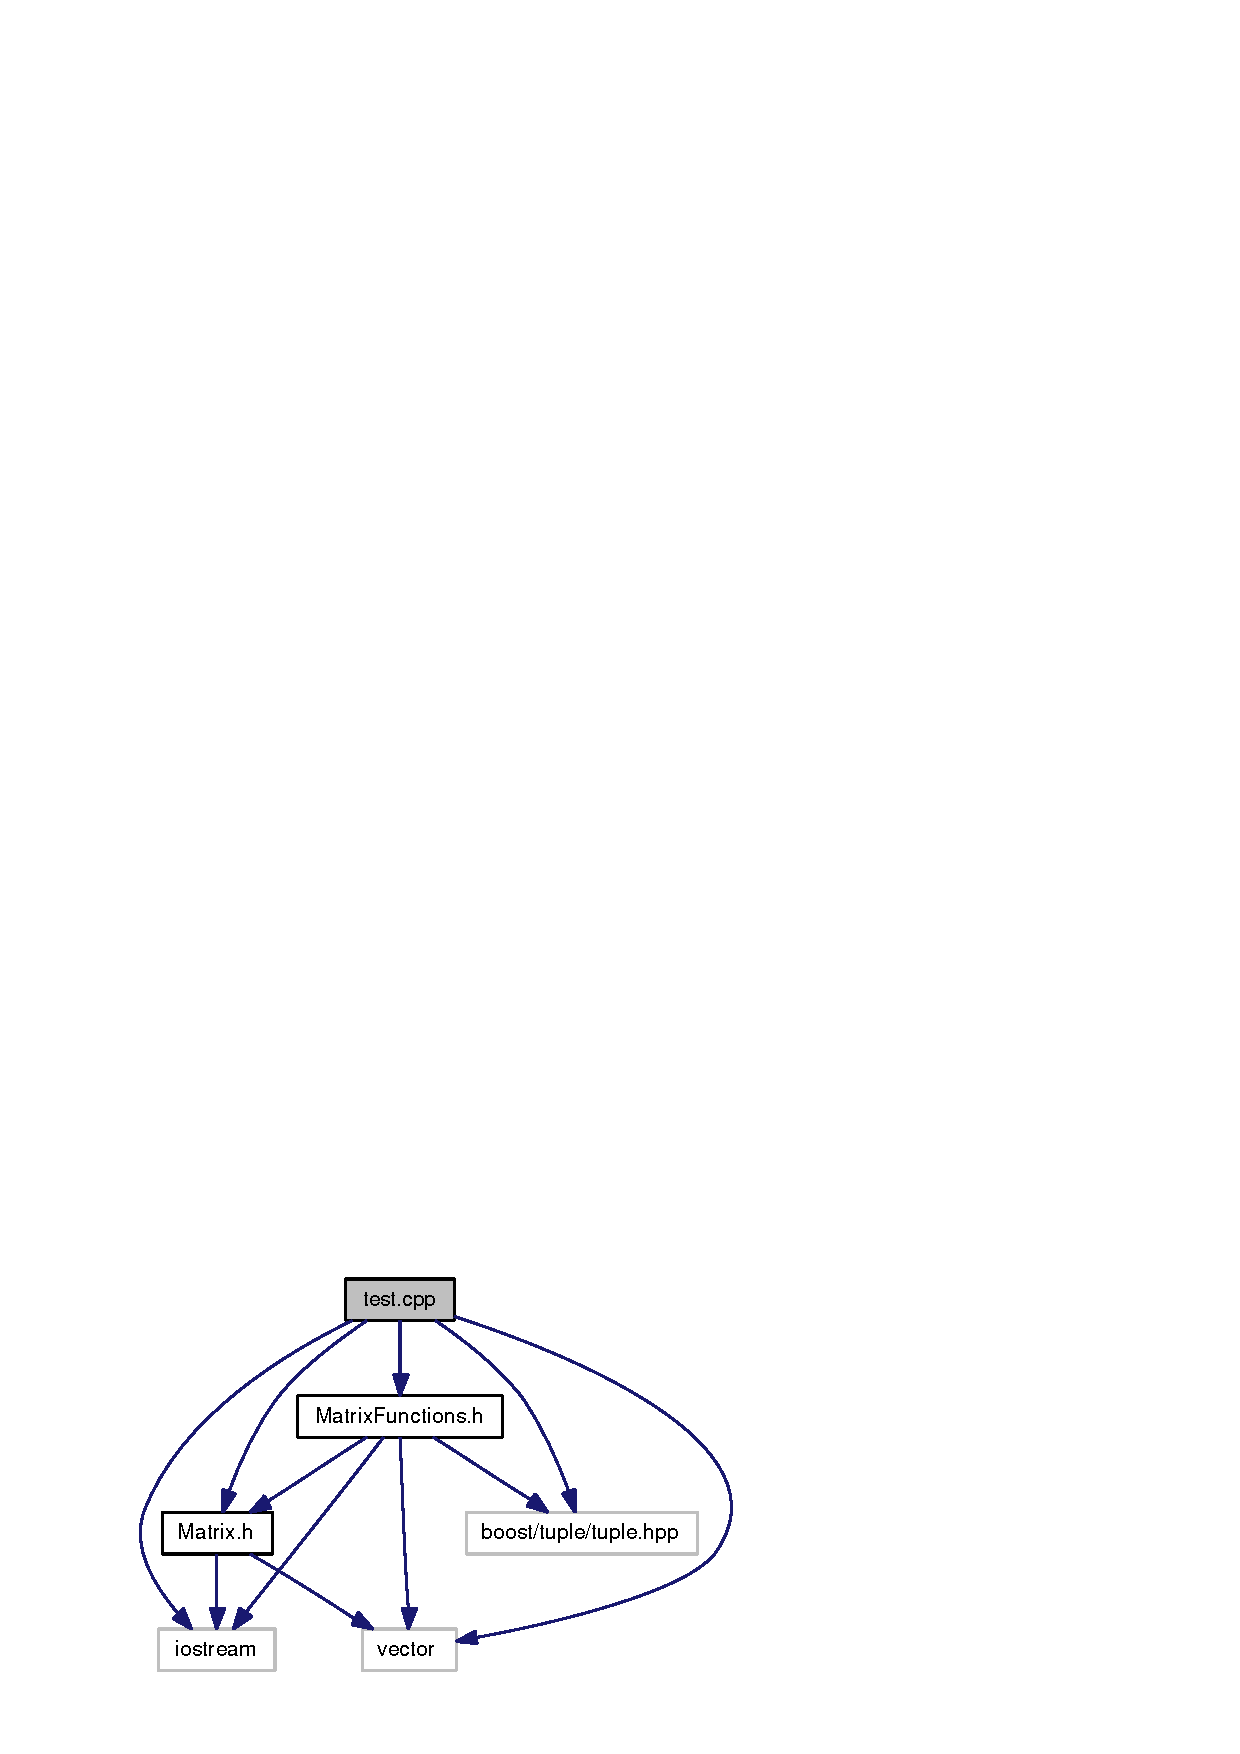
\includegraphics[width=270pt]{test_8cpp__incl}
\end{center}
\end{figure}
\subsection*{Functions}
\begin{DoxyCompactItemize}
\item 
int \hyperlink{test_8cpp_a0ddf1224851353fc92bfbff6f499fa97}{main} (int argc, char $\ast$argv\mbox{[}$\,$\mbox{]})
\end{DoxyCompactItemize}


\subsection{Function Documentation}
\hypertarget{test_8cpp_a0ddf1224851353fc92bfbff6f499fa97}{
\index{test.cpp@{test.cpp}!main@{main}}
\index{main@{main}!test.cpp@{test.cpp}}
\subsubsection[{main}]{\setlength{\rightskip}{0pt plus 5cm}int main (int {\em argc}, \/  char $\ast$ {\em argv}\mbox{[}$\,$\mbox{]})}}
\label{test_8cpp_a0ddf1224851353fc92bfbff6f499fa97}

\printindex
\end{document}
